\documentclass[tikz,border=10pt]{standalone}
\usetikzlibrary{arrows.meta, positioning, calc}
\usepackage{amssymb}

\begin{document}
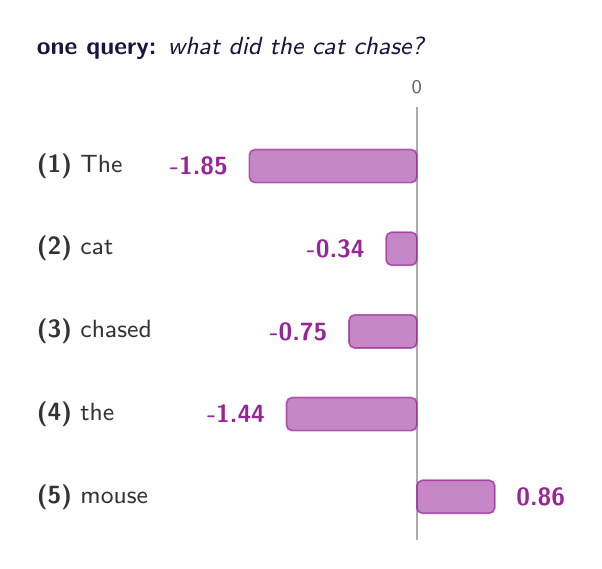
\begin{tikzpicture}[
    every node/.style={font=\sffamily},
]

% ---------------------------------------------------------------- colours
\definecolor{c1}{HTML}{15173D}   % the query
\definecolor{c2}{HTML}{982598}   % the scores
\definecolor{c3}{HTML}{E491C9}
\definecolor{c4}{HTML}{F1E9E9}
\definecolor{axiscolor}{HTML}{333333}
\definecolor{labelcolor}{HTML}{6B6472}

% ================================================================
% Diverging bars so the sign of each score is visible at a glance.
%   zero line  x = 4.2
%   scale      1.15 units of x per 1.0 of score
%   rows       y = 5.0, 3.95, 2.9, 1.85, 0.8
% ================================================================

\def\zero{4.2}
\def\sc{1.15}

\node[font=\sffamily\small, text=c1, anchor=west] at (-0.75, 6.5)
    {\textbf{one query:} \emph{what did the cat chase?}};

% zero line
\draw[labelcolor, opacity=0.55, line width=0.7pt] (\zero, 0.25) -- (\zero, 5.75);
\node[font=\sffamily\scriptsize, text=labelcolor, anchor=south] at (\zero, 5.8) {0};

% word / y / score
\foreach \w/\y/\s in {%
    {\textbf{(1)} The}/5.0/-1.85,
    {\textbf{(2)} cat}/3.95/-0.34,
    {\textbf{(3)} chased}/2.9/-0.75,
    {\textbf{(4)} the}/1.85/-1.44,
    {\textbf{(5)} mouse}/0.8/0.86%
} {
    \node[font=\sffamily\small, text=axiscolor, anchor=west] at (-0.75, \y) {\w};

    \fill[c2, opacity=0.55, rounded corners=2pt]
        (\zero, \y-0.21) rectangle (\zero + \s*\sc, \y+0.21);
    \draw[c2, opacity=0.7, line width=0.6pt, rounded corners=2pt]
        (\zero, \y-0.21) rectangle (\zero + \s*\sc, \y+0.21);
}

% the numbers, placed on the far side of each bar from the zero line
\node[font=\sffamily\small\bfseries, text=c2, anchor=east] at (\zero - 1.85*\sc - 0.15, 5.0) {-1.85};
\node[font=\sffamily\small\bfseries, text=c2, anchor=east] at (\zero - 0.34*\sc - 0.15, 3.95) {-0.34};
\node[font=\sffamily\small\bfseries, text=c2, anchor=east] at (\zero - 0.75*\sc - 0.15, 2.9) {-0.75};
\node[font=\sffamily\small\bfseries, text=c2, anchor=east] at (\zero - 1.44*\sc - 0.15, 1.85) {-1.44};
\node[font=\sffamily\small\bfseries, text=c2, anchor=west] at (\zero + 0.86*\sc + 0.15, 0.8) {0.86};

% the takeaway lives in the figcaption, not inside the figure

\end{tikzpicture}
\end{document}
